%%%%%%%%%%%%%%%%%%%%% RJT TeX Template %%%%%%%%%%%%%%%%%%%%%
\documentclass[twoside,11pt,a4paper]{article}

%%%% BHAM PREAMBLE - SET THIS FIRST! %%%%
\newcommand{\bhamstudentname}{Sarathkumar Padinjare Marath Sankaranarayanan}
\newcommand{\bhamthesistitle}{Machine Learning \& Deep Learning Approaches to Predict Credit Card Default}
\newcommand{\bhamfronttitle}{Machine Learning \& Deep Learning Approaches \\ to Predict Credit Card Default}
\newcommand{\bhamschool}{School of Computer Science}
\newcommand{\bhamcollege}{Engineering and Physical Sciences}
\newcommand{\bhamdegree}{MSc. Artificial Intelligence \& Computer Science}
\newcommand{\bhamid}{2359859}
\newcommand{\bhamsupervisor}{Dr.Kashif Rajpoot}
\newcommand{\bhamyear}{2022}
%%%%           %%%%


\usepackage[hyphens]{url}
\usepackage[breaklinks]{hyperref}
\usepackage{fancyhdr}
\usepackage[sort]{natbib} 
\usepackage{comment} % from http://www.latex-community.org/forum/viewtopic.php?f=5&t=4538
\usepackage{dirtree} % from http://blog.plenz.com/2011-07/represent-directory-structures-in-latex.html
\usepackage{longtable} % from http://stackoverflow.com/questions/2896833/how-to-stretch-a-table-over-multiple-pages
\usepackage{algorithm}   
\usepackage{algorithmic}   %both algorithm* from http://hasini-gunasinghe.blogspot.co.uk/2014/02/presenting-algorithmsprotocols-in-neat.html

\renewcommand{\algorithmiccomment}[1]{#1} %http://tex.stackexchange.com/q1uestions/61861/algorithmic-package-for-loop-and-comment-at-the-same-line
\usepackage[printonlyused]{acronym}
\usepackage[table]{xcolor}
\usepackage{subcaption}

\pagestyle{fancy}
\renewcommand{\sectionmark}[1]{\markboth{#1}{}}	%from tex.stackexchange.com/questions/111361

\lfoot{\bhamstudentname}
\cfoot{}
\rfoot{}
\fancyhfoffset[L]{0cm} %this fixes the right page number margin issue.
\newcommand{\HRule}{\rule{\linewidth}{0.5mm}}
\renewcommand{\headrulewidth}{0pt}
\newcommand{\tab}{\hspace*{1.25em}}
\newcommand{\minitab}{\hspace*{0.25em}}

%footnote stuff
\usepackage{perpage}
\MakePerPage{footnote} %the perpage package command
\renewcommand*{\thefootnote}{\fnsymbol{footnote}}

\lhead{}\chead{}\rhead{}
\setlength{\headheight}{28pt} %fixes the warnings about headheight being too small
\setlength{\headsep}{6pt}
\pdfoutput=1 % we are running PDFLaTeX
\usepackage[left=2.55cm,right=1.6cm,top=1.8cm,bottom=1.8cm]{geometry}
\usepackage{titling}	
\setlength{\droptitle}{-2.75cm}   % This is your set screw\\
\usepackage{titlesec}
\titleformat*{\section}{\normalsize	\bfseries}
\titleformat*{\subsection}{\small \bfseries}
\titleformat*{\subsubsection}{\footnotesize \bfseries}
%modifies the size of the gaps between the top of the title and bottom
% arguments {type}{left}{top}{bottom}
\titlespacing*{\section} {0pt}{3ex plus 1ex minus .2ex}{2ex plus .2ex}
\titlespacing*{\subsection} {0pt}{2.25ex plus 1ex minus .2ex}{0.75ex plus .2ex}
\titlespacing*{\subsubsection}{0pt}{2.ex plus 1ex minus .2ex}{0.5ex plus .2ex}

\setlength{\intextsep}{0pt} %from http://tex.stackexchange.com/questions/25828/how-to-remove-change-the-vertical-spacing-before-and-after-an-algorithm-environ

\usepackage[pdftex]{graphicx}
\graphicspath{ {figures/} }

\usepackage{enumitem}
\usepackage{pdfpages}
\usepackage{lastpage}
\usepackage{amsmath}
\usepackage{amsfonts}
\usepackage{amssymb}


\usepackage{epstopdf} %http://dirkraffel.com/2007/11/19/include-eps-files-in-latex/comment-page-2/

\usepackage{listings}
\lstset{
 basicstyle=\ttfamily,
  columns=fullflexible,
  keepspaces=true,
breaklines=true
} %from http://tex.stackexchange.com/questions/121601/automatically-wrap-the-text-in-verbatim

\newcommand{\todo}[1]{\textcolor{red}{TODO: #1}\PackageWarning{TODO:}{TODO found: #1!}} %from http://tex.stackexchange.com/questions/9796/how-to-add-todo-notes

\DeclareGraphicsExtensions{.jpg,.png}
%%%%%%%%%%%%%%%%%%%%%  END of TEMPLATE %%%%%%%%%%%%%%%%%%%%%

\title{MSc. Project\\\bhamthesistitle}
\author{\textsf{\bhamstudentname {\textsf{}}}}

\date{}
\begin{document}

\pagenumbering{gobble} % fix at	 http://tex.stackexchange.com/questions/7355/how-to-suppress-page-number
% this came from http://en.wikibooks.org/wiki/LaTeX/Title_Creation and http://tex.stackexchange.com/questions/14778/error-with-hrule
\begin{titlepage}
\begin{center}
% this was from http://tex.stackexchange.com/questions/7219/how-to-vertically-center-two-images-next-to-each-other
\begin{minipage}{6in}
  \centering
  \raisebox{-0.5\height}{
\includegraphics[width=1.25in]{crest}}
  \hspace*{.2in}
  \raisebox{-0.5\height}{
\includegraphics[height=0.9375in]{uni}}
  \end{minipage}
  \\ [1.0cm]
\textsc{{\LARGE \bhamschool\\}College of \bhamcollege}\\[3.5cm]

\textsc{\Large MSc. Project}\\[0.5cm]

% Title
\HRule \\[0.4cm]
\begin{center}\Huge
\bhamfronttitle
\end{center}
\HRule \\[1.5cm]
% Team and Members

\begin{center}
Submitted in conformity with the requirements\\ for the degree of \bhamdegree\\
\bhamschool\\ University of Birmingham\\
\vspace{2cm}
\bhamstudentname \\
Student ID: \bhamid\\
Supervisor: \bhamsupervisor      
\end{center}
\vfill

% Bottom of the page
{\large September \bhamyear}

\end{center}
\end{titlepage}

\section*{\centering Abstract}	


% Taken from the MSc Thesis template, and edited for a PGT report
The material contained within this report has not previously been
submitted for a degree at the University of Birmingham or any other university.
The research reported within this report has been conducted by the author
unless indicated otherwise.\\
\\
\textbf{Keywords} Credit Card Default Prediction, Ensemble Learning

\vfill
\clearpage

\section*{\centering Declaration}
% Taken from the MSc Thesis template, and edited for a PGT report
The material contained within this report has not previously been
submitted for a degree at the University of Birmingham or any other university.
The research reported within this report has been conducted by the author
unless indicated otherwise.\\
\\
\textbf{Signed} Sarathkumar Padinjare Marath Sankaranarayanan 

\vfill
\clearpage
\begin{center}
\vspace*{\fill}
\begin{minipage}{6in}

%\centering \Large{``Most men who have really lived have had, in some share, their great adventure.\\This railway is mine."}\\{\normalsize{\textsc{James J. Hill}}, \emph{Railway Pioneer}} \vspace{2cm}

%\centering \Large{``Steam engines don't answer back.\\ You can belt them with a hammer and they say nowt."}\\{\normalsize{\textsc{Fred Dibnah}}, \emph{Steeplejack and Engineer}} \vspace{2cm}

\centering \Large{``You have to learn the rules of the game.\\ And then you have to play better than anyone else"}\\{\normalsize{\textsc{Albert Einstein}}}

  \end{minipage}
  \vspace*{\fill}
\end{center}


\clearpage
\maketitle
\vspace{-5.5em} %fixes distance between \maketitle and the TOC
\begingroup
    \fontsize{9pt}{11pt}\selectfont
\tableofcontents
\endgroup
\clearpage
\phantomsection
\section*{Table of Abbreviations}

\normalsize
\begin{acronym}[SCEPTICS] % Give the longest label here so that the list is nicely aligned
\acro{SVM} {Support Vector Machine}
\acro{ANN} {Artificial Neural Network}
\acro{GBDT} {Gradient Boosting Decision Tree}
\acro{GRU} {Gated Recurrent Unit}
\acro{LGBM} {Light Gradient Boosting Machine}
\acro{XGBoost} {Xtreme Gradient Boosting Machine}
\acro{GRU} {Gated Recurrent Unit}
\acro{CV}{Cross Validation}
\acro{SMOTE}{Synthetic Minority Oversampling Technique}
\acro{RAM}{Random Access Memory}
\acro{MSE}{Mean Squared Error}
\acro{ReLU}{Rectified Linear Unit}
\acro{CFS}{Correlation Based Feature Selection}
\acro{AUC}{Area Under the Curve}
\acro{PCA}{Principle Component Analsys}
\acro{RNN}{Recurrent Neural Network}
\acro{RF}{Random Forest Classifier}
\acro{KNN}{K-Nearest Neighbours}
\acro{RBF}{Radial Basis Function}
\acro{DT}{Decision Tree Classifiers}
\acro{GOSS}{Gradient based One-side Sampling}
\acro{TP}{True Positive}
\acro{TN}{True Negative}
\acro{FP}{False Positive}
\acro{FN}{False Negative}
\end{acronym}


\addcontentsline{toc}{section}{Table of Abbreviations} 
\clearpage


\listoffigures

\addcontentsline{toc}{section}{List of Figures} 
\clearpage

\listoftables
\addcontentsline{toc}{section}{List of Tables} 
\clearpage

% set up the page numbering and counter - Table of Abbreviations has no page number
% also set up the footers and headers appropriately.
\pagenumbering{arabic}
\setcounter{page}{1}
\lhead{}\chead{MSc. Project Report :: \nouppercase{Section \thesection\minitab :: \leftmark}}\rhead{}
\rfoot{Page \thepage \hspace*{0.2pt} of \pageref{LastPage}}
\renewcommand{\headrulewidth}{0.4pt}

\section{Introduction}
This section will introduce the user to definitions of terms relevant for understanding the problem, discuss the motivation behind the problem, the aim \& approach taken to solve the problem, and the structure of this report. 


\subsection{Definitions}

\subsubsection{Credit Card Statement Date}
The credit card statement date is the date on which the statement/bill is generated every month. Any transaction conducted on the card post billing date will reflect in the next month's credit card statement.

\subsubsection{Delinquent Account}
A credit card account is considered delinquent if the customer has failed to make the minimum monthly payment for 30 days from the original due date.

\subsubsection{Delinquency Rate}
The percentage of credit card accounts within a financial institution's portfolio whose payments are delinquent.
\begin{equation}
	Delinquency Rate = \left(\frac{Number Of Delinquent Credit Card Accounts}{Total Number Of Credit Card Account}\right) * 100
\end{equation}

\subsubsection{Credit Card Default}
The customer is considered as defaulting customer in the event of nonpayment of the due amount in 120 days after the latest statement date.

\subsection{Motivation}
Delinquency rates \& credit card default rates are directly proportional. According to the  figure \ref{fig:fredgraph}, the delinquency rates were at an all-time high just before the recession started in 2008; moreover, this was the same time when more \& more customers began to default on credit card payments. 

Predicting credit defaults is essential for managing risk in the consumer lending industry. Credit default prediction enables lenders to make the best possible lending decisions, improving customer satisfaction and fostering strong company economics. \\

\begin{figure}[ht]
	\centering
	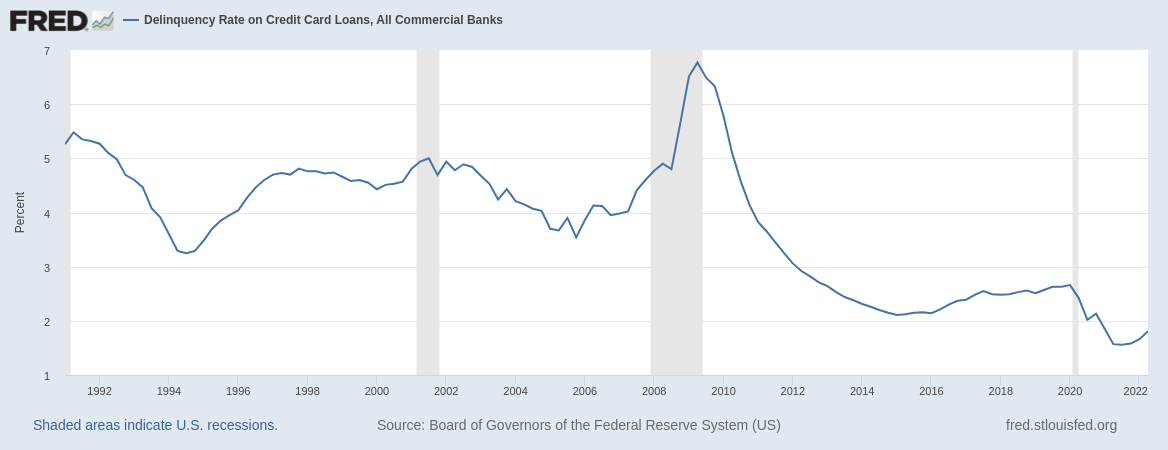
\includegraphics[width=1.0\textwidth]{fredgraph}
	\caption[Delinquency rate on credit card loans for the period 1992-2022]{Delinquency rate on credit card loans for the period 1992-2022{\citep{fedgraph_delinquency_history}}.}
	\label{fig:fredgraph}
\end{figure}

Existing models can be used to manage risk. However, developing models that perform better than those in use is feasible.

\subsection{Aim \& Approach}
The objective of this project was to explore different machine learning algorithms \& deep learning architectures on the American Express default prediction dataset\citep{amex-default-prediction-dataset} to predict if a customer will default on the payment in the future. The project work started by developing a model using classic machine learning algorithm \acf{SVM} followed by creating multiple models using Random Forest Classifier \& \acf{GBDT} algorithms. \acf{ANN}, \acf{GRU} \& Custom ensemble model created by model combining \acs{ANN}, \acs{GRU} and \acs{GBDT} were created as part of exploring deep learning architectures. Finally created a lean model, using less features \& optimzed parameters using \acs{GBDT} which provided comparable performances to the previously explored models.

\subsection{Structure of Report}
The remainder of the report is structured as follows: in Section \ref{sec:background_knowledge} background information on different machine learning \& deep learning algorithms along with metrics explanation is provided. Then in Section \ref{sec:literature_review} a literature review related to the credit card default prediction research is given. Section \ref{sec:materials} \& \ref{sec:methodology} provides detailed explanations on the dataset, tools \& software used in the project, and methodology followed for creating the models. Model evaluation results and the comparison is given in Section \ref{sec:results_discussions}. Finally Section \ref{sec:conclusion_summary} discusses the conclusion of the project. 

\vfill
\clearpage
\section{Background Knowledge} \label{sec:background_knowledge}
This section provides the reader with the required background information on the machine learning algorithms, deep learning architectures \& metrics.

\subsection{\acf{SVM}}
\subsection{Decision Tree}
\subsection{Ensemble Models}
\subsection{\acf{GBDT}}
\subsection{\acf{XGBoost}}
\subsection{\acf{LGBM}}
\subsection{\acf{ANN}}
\subsection{\acf{GRU}}
\subsection{Feature Selection - Select From Model}
\subsection{Ordinal Encoder}
\subsection{Class Imbalance}
\subsection{Data Oversampling}
\subsubsection{\acf{SMOTE}}
\subsubsection{KMeans \acs{SMOTE}}
\subsection{Metrics}
\subsubsection{Accuracy}
\subsubsection{F1-Score}
\subsubsection{Recall}
\subsection{\acf{CV}}
\subsection{Bias \& Variance }
\subsection{Hyper Parameter Tuning}
\subsubsection{Grid Search CV}
\subsection{Stochastic Gradient Descent}
\subsection{File Format}
\subsubsection{Parquet}
\subsection{Binary Cross Entropy}
\subsection{Summary}

\vfill
\clearpage
\section{Literature Review}\label{sec:literature_review}
\subsection{Introduction}
This section discusses the current techniques used to predict the credit card default. Since the dataset used for these studies differ, a direct comparison of results is not possible. However, an overall comparison of different techniques and its efficiency in predicting the credit card default will be discussed wherever possible.

\subsection{Previous Work}
\citep{sayjadah2018credit} developed logistic regression, rpart decision tree \& Random Forest Classifier models on dataset generated from credit card operations. The dataset contains 30000 records and 24 features. A \acf{CFS} technique was used to reduce the dimensionality of the dataset. 30\% of the dataset was used as the test set for evaluating the performance. \citep{sayjadah2018credit} found that the Random Forest Classifier provided highest \acf{AUC} among the models.\\

\citep{widyadhanacredit} developed Logistic Regressiion, \acs{SVM}, \acs{ANN} \& Random Forest Classifier models to preduct credit card default on dataset containing 1000 records and 11 features. The dataset contains credit card data from cardholders from the territory of Indonesia;moreover, the authors used \acf{PCA} to do feature selection also. The dataset is split into 70:30 Train/Test set and the \acs{AUC} was used to compare the results. The authors found that the Random Forest Classifier outperformed all other models by far and provided a 80\% \acs{AUC} score.\\

\citep{hsu2019enhanced} approached the credit card default prediction from a different perspective and proposed a model where dynamic features (time dependent features) were first passed through a \acf{RNN} network to extract the time dependent features. Then the extracted dynamic features were concatenated with the static features and trained on a Random Forest Classifer. The dataset contained 30,000 samples credit card payment history with 23 features (5 static feature, 18 dynamic features). The authors compared the results of the proposed model with the \acs{SVM}, Logistic Regression and KNN models and found that proposed method outperformed the others and provided a \acs{AUC} score of 78\%.

\citep{alam2020investigation} investigated different approaches to solve the credit card default prediction problem with a specific focus on Class Imbalance. The credit card default prediction dataset are inherently imbalanced as only a small fraction of customers default on credit card. The authors employed different data under/over sampling techniques and evaluated performance on multiple credit card default dataset. They found that \acs{GBDT} classifier when used with KMeans \acs{SMOTE} provided the best results and the models performed significantly better on balanced datasets compared to imbalanced datasets.

\citep{faraj2021comparison} research shows that ensemble  methods  consistently  outperform  Neural  Networks  and  other  machine  learning algorithms in terms of F1 score. \citep{faraj2021comparison} uses the same dataset as the \citep{sayjadah2018credit} which has 30,000 records and 24 features. The authors found that \acs{XGBoost} provided maximum F1 score compared to Neural Networks, Random Forest Classifier and custom ensemble stacking model. Authors also concludes that the performance of \acs{XGBoost} model did not improve on balanced datasets. This observation was in contrary to the observations made by \citep{emil2019enhancing}, the authors of earlier had found that the best performance is achieved on \acs{GBDT} with KMeans \acs{SMOTE} method.

\subsection{Summary}
In conclusion, the ensemble boosting models generally provided better performance than the classic machine learning and deep learning techniques. The data under/over sampling had mixed performances depending on the dataset, some performed better with under/over sampling and some did not. Out of data under/over sampling techniques, KMeans \acs{SMOTE} performed better. Some studies used feature selection techniques in the data preprocessing techniques which improved the model efficiency. The studies discussed in the section used dataset which were imbalanced and  contained atmost 30,000 records; however, \citep{amex-default-prediction-dataset} contains 5 Million records and exploring the different techniques on such large scale dataset will help us to consolidate the understanding gained from these papers.

\vfill
\clearpage
\section{Materials}\label{sec:materials}

\subsection{Primary Dataset}
The primary dataset contains 190 aggregated profile features of 458913 American Express customers at each statement date for 13 months. Features are anonymized and normalized, and fall into the following general categories:

\begin{itemize}
	\item D\_* = Delinquency variables
	\item S\_* = Spend variables
	\item P\_* = Payment variables
	\item B\_* = Balance variables
	\item R\_* = Risk variables	
\end{itemize}

This dataset\citep{amex-default-prediction-dataset} was released as part of the "American Express - Default Prediction" hosted in Kaggle by the American Express team.

\subsection{Secondary Dataset}
The secondary dataset was derived from primary dataset by applying the below mathematical aggregate operations to the numerical features.
\begin{itemize}
	\item Minimum 
	\item Maximum
	\item Mean
	\item Last Value
	\item Standard Deviation
\end{itemize}

Aggregate for the categorical features were taken by the applying below operations.
\begin{itemize}
	\item Last Value
	\item Count
	\item Unique Value Count
\end{itemize}

The secondary dataset contains 920 features and 458913 records.

\subsection{Tools \& Software}
The primary programming language used for the implementation of this project is Python version 3.7. Data analysis and manipulation is done using Pandas(1.3.5), seaborn(0.11.2) \& Dask(2.12.0) packages. Scikit Learn(1.0.2) package is used for create, train \& evaluate machine learning models. \acs{ANN} \& \acs{GRU} models were created using Tensorflow (2.8.2).Google colab was used to train the model in cloud and Github was used as the version control \& project management software.

\vfill
\clearpage
\section{Methodology}\label{sec:methodology}
\subsection{Introduction}
This section will first provide a brief overview of the overall strategy of the experiments performed as part of this project followed by  providing detailed explanation on the data preprocessing techniques used. Then in subsequent sections each experiment/model will be presented along with the model specific explanations \& details.

\subsection{Overview of Methodology Followed}
Figure \ref{fig:methodology} represents a overview of methodology in general followed for conducting experiments. The dataset was first split into chunks and stored in different files in parquet format to optimize the memory usage. Then, dataset was preprocessed to remove invalid values and encode categorical text variables to numerical values. Followed by data pre-processing, the dataset was split into Training \& Test set, this ensures that none of the entries in test set will have an influence in model training and model selection process. Then the dataset was enhanced using oversampling techniques to resolve the class imbalance issue;in addition, feature selection techniques were used to eliminate the features from the dataset which were less important and hence contribute very little to model. 
\begin{figure}[ht]
	\centering
	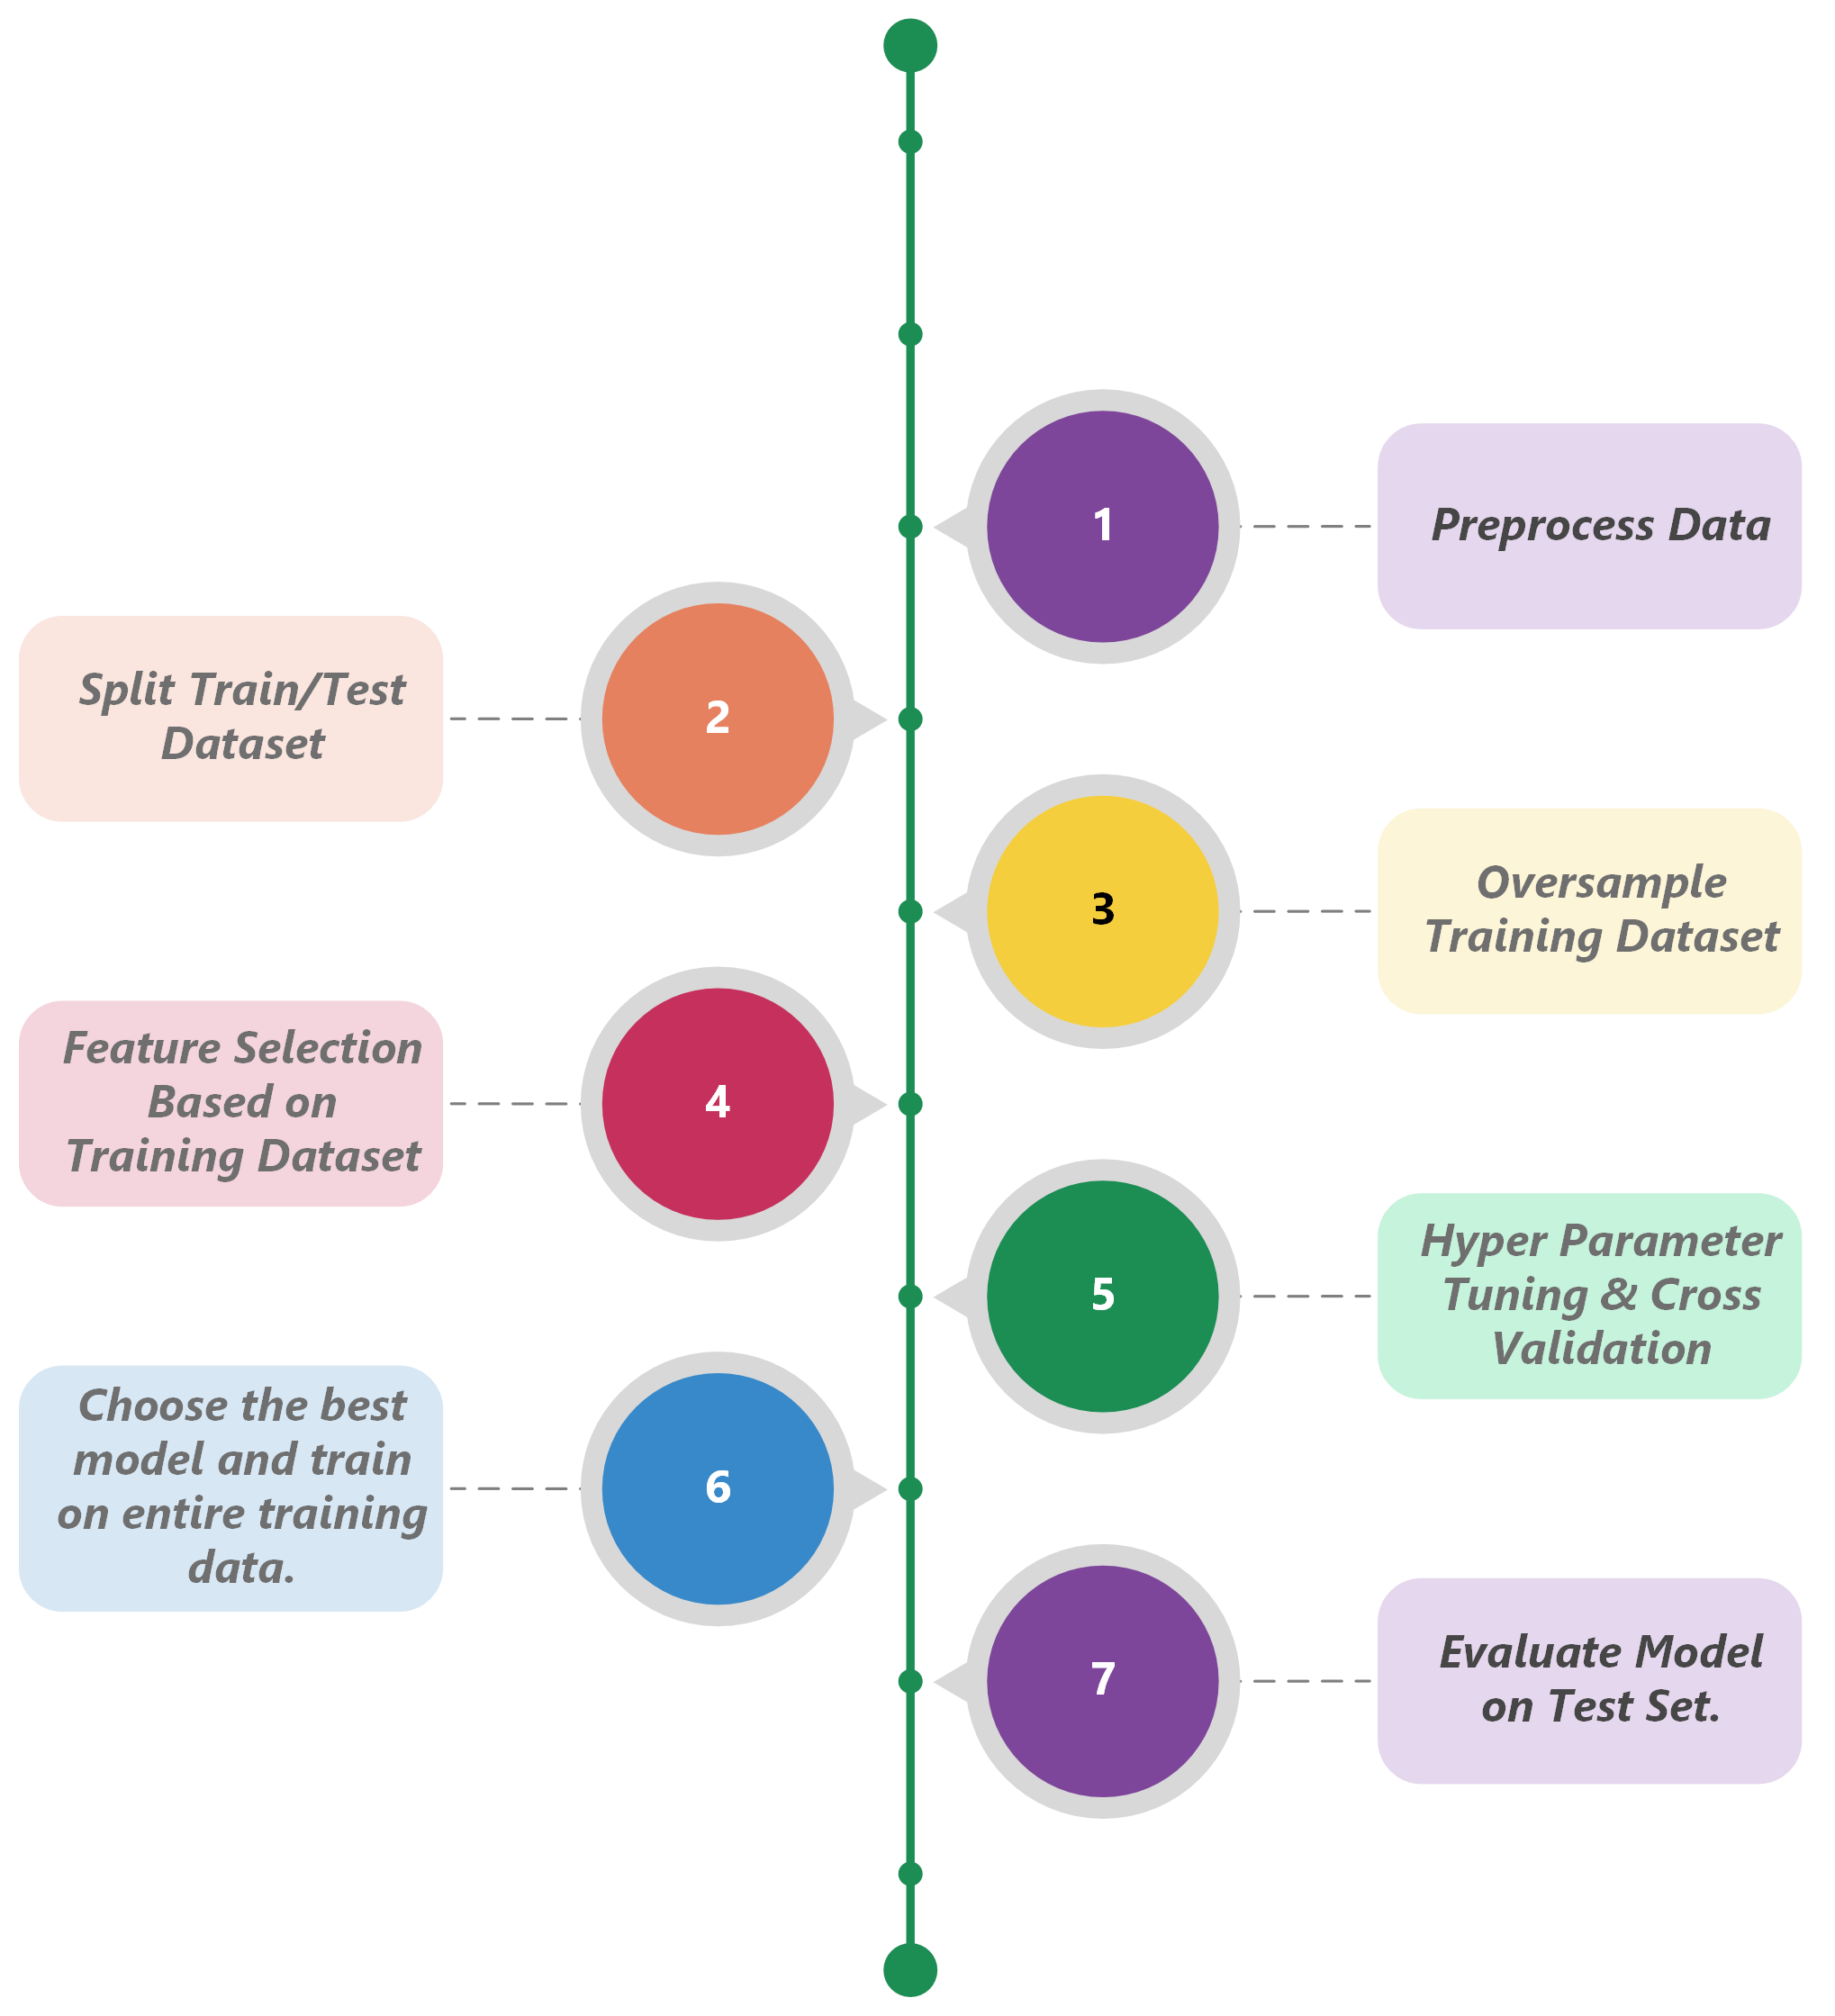
\includegraphics[width=1.0\textwidth, height=0.5\textheight]{methodology}
	\caption[Methodology]{Methodology followed for the experiments}
	\label{fig:methodology}
\end{figure}

After the feature selection, the model was created and then passed through a Hyperparameter tuning pipeline which helps to find the best parameters for the model which would give highest cross validation score. Finally the entire training dataset was trained on the best model found using hyperparameter tuning and the model was evaluated using the test set set aside at the beginning of the experiment.

\subsection{Data Preprocessing} 
This section discusses the common preprocessing techniques used in all experiments conducted as part of the project. The model specific data preporcessing techniques used will be discussed in respective sections describing the model.

\subsubsection{Default Values}
NaN \& NULL values in the dataset was replaced by Zero and if a column contains all values same, it was removed from the dataset. -1 was used as the default value for the categorical variables. The categorical variables were encoded using Ordinal Encoder before passing to the model training pipeline.

\subsubsection{Normalization}
The primary dataset from American Express is already normalized and all the values lies between zero to ten, hence none of the data normalization techniques were used to preporcess the data.
\subsubsection{Handling Memory Issue}
Google Colab provides 24 GB of \acf{RAM} in the  virtual environment, though the Primary Dataset is 16 GB,  the pandas library was unable to load the complete data into memory due to memory leakage issue in the framework. Dask library, which uses multiple Pandas dataframe under the hood, was used to overcome the memory. Dataframe API in Dask library splits the dataset into multiple chunks and loads each chunk on a need basis only ( Lazy Loading), this ensured that the complete 16 GB dataset could be loaded even at a low memory of 4GB.

Additionally, the primary dataset was loaded using Dask framework and split the dataset month wise, ie one file for each month. The month wise files were saved in parquet format which helped to reduce the total size of the dataset from 16GB to 7GB. Similarly the primary dataset was also split customer wise, ie 1-50000 customers data in one file, 50001-100000 customers data in second file etc. These files were later used to build the Secondary Dataset.

\subsection{Model 1 - \acf{SVM}}
The \acs{SVM} model was created with parameters Regularziation Term = L2 Norm(Squared Error Loss), Alpha = 0.0001, Loss='hinge'(soft-margin), tolerance=0.001. The primary dataset was used to train the model and the model converged after 28 iterations. Early stopping was used to prevent overfitting of the model and 10\% of the data from training set used as the validation set. Stochastic gradient descent was used to optimize the objective function, this ensured that even though the dataset contains millions of records, the training is able to proceed and finish in reasonable time.  20\% of the Secondary Dataset was used as test set to evaluate the performance of the model.
\subsection{Model 2 - Random Forest Classifier}
The Random Forest Classifier model uses 100 Decision Trees trained in parallel on the primary dataset. Each decision tree uses a different subset of Primary Dataset with maximum number of records in a database set to 600,000. Gini impurity metric is used to measure the quality of the split while building decision tree. Finally the model predicts the target variable by taking mean of all the predictions from the 100 individual decision trees. 20\% of the Secondary Dataset was used as test set to evaluate the performance of the model.
\subsection{Model 3 - \acf{GBDT}}
\acs{GBDT} model was created using 100 Decision Trees trained sequentially on the primary dataset. Friedman \acf{MSE} is used to measure the quality of a split; additionally, model was set to use only 60\% of the data for constructing each decision trees to avoid memory leakage issue. 10\% of the training set was set for validation purpose; furthermore, the parameters were set to stop the training if the validation score does not improve to avoid overfitting. Loss function for the training was set to Deviance. 20\% of the Secondary Dataset was used as test set to evaluate the performance of the model.
\subsection{Model 4 - \acf{XGBoost}}
\acs{XGBoost} model was created using training 100 base learners on the Secondary Dataset and each base learner is constructed using 80\% of the training dataset. Instead of using complete features to construct the base learner, parameters were set to use only 60\% of features, this helped to eliminate the memory leakage/overflow issues while training. Moreover, L2 regularization parameter was set to 0.9 to reduce the overfitting of the model. 20\% of the Secondary Dataset was used as test set to evaluate the performance of the model.

\subsection{Model 5 - \acf{LGBM}}
\acs{LGBM} model was trained on Secondary dataset and the 100 base learners were constructed using the entire features \& training set. Tradition Gradient Boosting Decision Trees were used as the boosting type and learning rate was set to 0.1. 20\% of the dataset were set aside as the test set for evaluating the model. Maximum depth is not set as to allow trees of any depth. 

\subsection{Model 6 - \acf{ANN}}
Figure \ref{fig:nn_arch} depicts the architecture of the custom \acs{ANN} model developed.  The primary dataset was first split into training \& test dataset, followed by oversampling the training dataset using KMeans \acs{SMOTE} to make the percentage of defaulting \& non defaulting customers equal. Then the training dataset was trained using the custom \acs{ANN} model. The first \& second layer uses \acf{ReLU} as the activation function, however the final layer uses Sigmoid as the activation function. Adam optimizer was used to optimze the objective binary cross entropy loss function. The trained model was tested and evaluated on the test set.\\
\begin{figure}[ht]
	\centering
	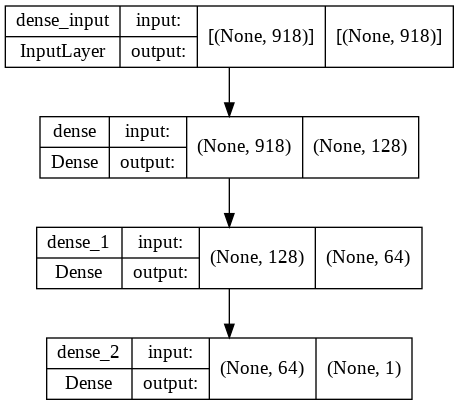
\includegraphics[width=0.6\textwidth, height=0.3\textheight]{nn_arch}
	\caption[Custom Neural Network Architecture]{Custom Neural Network Architecture}
	\label{fig:nn_arch}
\end{figure}

\subsection{Model 7 - \acf{GRU}}
Figure \ref{fig:gru_arch} represents the architecture of the GRU based model for predicting credit card default. The primary dataset is used for training this model;furthermore, the tanh function is used as the activation function and sigmoid  is used as the recurrent activation function  for the GRU layer. Dropout of 10\%, recurrent dropout of 50\% added to reduce the overfitting problem. The output of the GRU layer is then fed to dense layer followed by another dense layer with activation sigmoid for making final prediction. Optimizer used is Adam \& the loss function is Binary Cross Entropy. A dataset generator was created to provide input to the model in chunks, this helped to eliminate the memory issues while training. The final model contains 49165 trainable parameters.\\

\begin{figure}[ht]
	\centering
	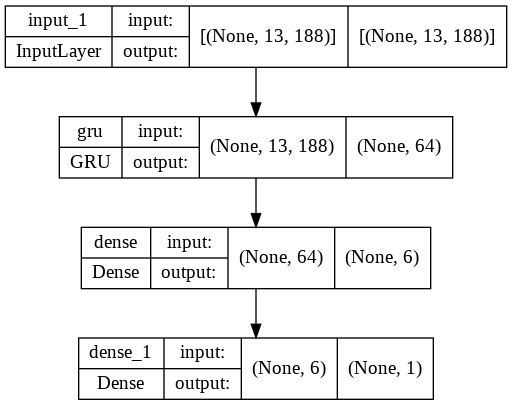
\includegraphics[width=0.6\textwidth, height=0.3\textheight]{gru_arch}
	\caption[GRU Model Architecture]{GRU Model Architecture\\}
	\label{fig:gru_arch}
\end{figure}
\subsection{Model 8 - Ensemble Stacking Model using \acs{ANN} + \acs{GRU} + \acs{GBDT}}
Figure \ref{fig:gru_nn_gbdt_arch} partially depicts the architecture of the custom ensemble stacking model. The primary dataset is first trained using \acs{GRU} layer followed by a dense layer. In parallel, the secondary dataset is trained using a 2 dense layers. Then the output of these two parallel legs were combined to form the concatenation layer. The output of concatenation layer is then trained using a  \acs{GBDT} model to get the final prediction. Adam optimizer was used to optimze the objective binary cross entropy loss function. Instead of loading complete dataset into memory and train the entire dataset in one go, a dataset generator was written to return chunks of data for training, this helped to eliminate the memory overflow issues.\\
\begin{figure}[ht]
	\centering
	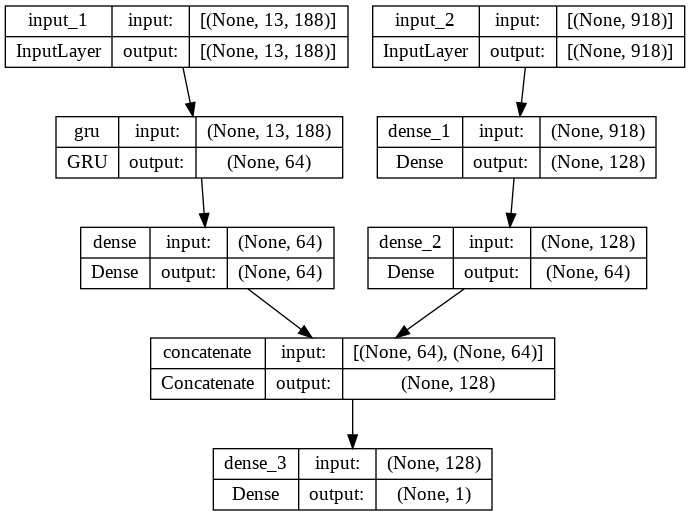
\includegraphics[width=0.7\textwidth, height=0.3\textheight]{GRU_NN_GBDT_Architecture}
	\caption[Custom Ensemble Stacking Model Architecture]{Custom Ensemble Stacking Model Architecture}
	\label{fig:gru_nn_gbdt_arch}
\end{figure}
\subsection{Model 9 - Lean \acs{LGBM} Model}
Finally, a lean model was created using \acs{LGBM} model which peformed on par with the other models but with less resources \& data. Firstly the 20\% of the dataset was set aside as test set and remaining 80\% for training purpose. Training dataset was then oversampled using KMeans \acs{SMOTE} method which resulted in the number of defaulting customers \& non defaulting customers to become equal. Secondly the the training dataset was trained using a simple \acs{SVM} model to extract the feature importances; in addition, the features with feature importance weight less than the mean of importance of weights were discarded. This helped to reduced the feature count from 920 in the secondary dataset to 279. This modified dataset was then passed through a Grid Search CV pipeline to choose the best parameters for maximum depth \& maximum number of leafs for base learner trees, and boosting type. \acf{CV} Recall score was used as the metric to choose the best model. Finally, a \acs{LGBM} model was created using the best model parameters found using GridSearchCV and trained the same on the complete training dataset. The final model was tested and evaluated on the test set.

\subsection{Summary}
Firstly, this section presented overall methodology followed for the experiments followed by the data preprocessing techniques used. Handling of invalid feature values, normalization \& handling memory leakage and memory overflow issue were discussed in the Data Preprocessing section. Secondly, the 9 different models created to solve the problem were discussed. Initially \acs{SVM} model \& Random Forest Classifier model were discussed followed by more advanced machine learning techniques such as \acs{GBDT}, \acs{XGBoost} \& \acs{LGBM}. Then 3 models using deep learning techniques such as Neural Network, \acs{GRU}  and Ensemble Stacking model were presented. Finally a lean model was developed and presented which used less features for training, was computationally less expensive and was explainable model. Before training the final model, the model was passed through a data oversampling pipeline, feature selection pipeline. The model was also tuned using GridSearchCV method to find the optimal hyper parameters. In all the experiments 20\% of data was set aside before training for testing \& evaluation purposes.

\vfill
\clearpage
\section{Results \& Discussions}\label{sec:results_discussions}
\begin{table}
	\begin{center}
		\begin{tabular}{|| c | c | c | c | c ||} 
			\hline
			Model & F1 Score & Recall & Accuracy & Precision \\ [0.5ex] 
			\hline\hline
			SVM	 & 74.66	& 75.57	& 87.24	& 73.78 \\
			\hline
			RF	 & 73.81	& 72.78	& 87.13	& 74.86 \\
			\hline
			GBDT	 & 74.33	& 74.13	& 87.25	& 74.52 \\
			\hline
			XGBoost	 & 80.22	& 80.11	& 89.79	& 80.34 \\
			\hline
			LGBM	 & 81.01	& 81.11	& 90.13	& 80.91 \\
			\hline
			ANN	 & \cellcolor[HTML]{339933} 81.03	&  \cellcolor[HTML]{339933} 81.81	& 90.09	& 80.27 \\
			\hline
			GRU	 & 79.81	& 79.96	& 90.67	& 79.65 \\
			\hline
			GRU+ANN+GBDT	 & 80.09	& 79.71	& \cellcolor[HTML]{339933} 90.87	& 80.49 \\
			\hline
			Lean LGBM	 & 80.95	& 80.68	& 90.15	& \cellcolor[HTML]{339933} 81.23 \\
			\hline
		\end{tabular}
		\caption{Comparison of metrics on various models.}
		\label{table:results}
	\end{center}
\end{table}

\begin{table}
	\begin{center}
		\begin{tabular}{|| c | c ||} 
			\hline
			Model & Trainable Parameters \\ [0.5ex] 
			\hline\hline
			ANN	& 125,953 \\
			\hline
			GRU	& 49,165 \\
			\hline
			GRU+ANN+GBDT	& 178,945 \\
			\hline
		\end{tabular}
		\caption{Trainable parameters comparison of Deep Learning Models}
		\label{table:trainable_params}
	\end{center}
\end{table}


\begin{figure}[ht]
	
	\begin{subfigure}{0.4 \textwidth}
		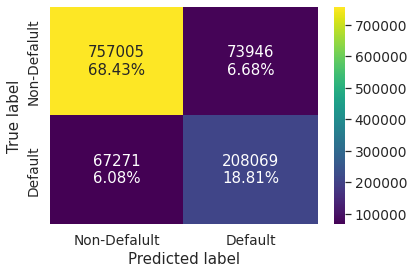
\includegraphics[width=1\linewidth, height=0.8\linewidth]{cm_svm}
		\subcaption[Support Vector Machine]{\acs{SVM}}
		\label{fig:cm_svm}
	\end{subfigure}
	\hfill
	\begin{subfigure}{0.4 \textwidth}
		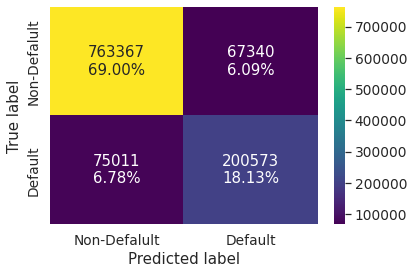
\includegraphics[width=1\linewidth, height=0.8\linewidth]{cm_rf}
		\caption[Random Forest]{\acs{RF}}
		\label{fig:cm_rf}
	\end{subfigure}
	\begin{subfigure}{0.4 \textwidth}
		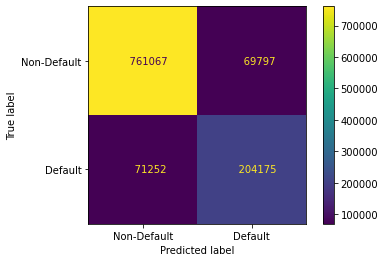
\includegraphics[width=1\linewidth, height=0.8\linewidth]{cm_gbdt}
		\caption[Gradient Boosting Decision Tree]{\acs{GBDT}}
		\label{fig:cm_gbdt}
	\end{subfigure}
	\hfill
	\begin{subfigure}{0.4 \textwidth}
		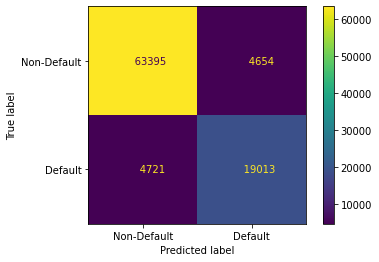
\includegraphics[width=1\linewidth, height=0.8\linewidth]{cm_xgboost}
		\caption[Xtreme Gradient Boosting Descision Tree]{\acs{XGBoost}}
		\label{fig:cm_xgboost}
	\end{subfigure}
	\begin{subfigure}{0.4 \textwidth}
		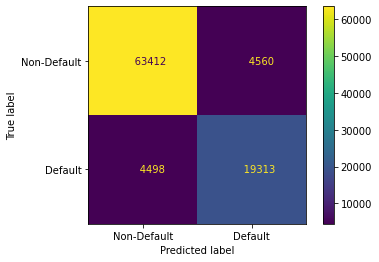
\includegraphics[width=1\linewidth, height=0.8\linewidth]{cm_lgbm}
		\caption[Light Gradient Boosting Machine]{\acs{LGBM}}
		\label{fig:cm_lgbm}
	\end{subfigure}
	\hfill
		\begin{subfigure}{0.4 \textwidth}
		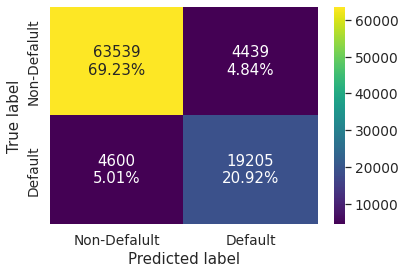
\includegraphics[width=1\linewidth, height=0.8\linewidth]{cm_lean_lgbm}
		\caption[Lean Light Gradient Boosting Machine]{Lean LGBM}
		\label{fig:cm_lean_lgbm}
	\end{subfigure}
	\caption[Confusion Matrix of Machine Leaning Models]{Confusion Matrix of Machine Leaning Models}
	\label{fig:cm_ml}
\end{figure}
\subsection{Summary}
dfsadfsd

\vfill
\clearpage
\section{Conclusion \& Summary}\label{sec:conclusion_summary}
asfsf
\subsection{Summary}
dfsadfsd

\vfill
\clearpage

\lhead{}\chead{MSc. Project Report :: \nouppercase{\leftmark}}\rhead{}
\phantomsection
\addcontentsline{toc}{section}{References}
\bibliographystyle{agsm} 
\bibliography{mybib}

\clearpage

\section{Appendix One: Code}

\subsection{Directory Structure} 

\subsection{Running the Provided Code}

\clearpage
\end{document}

